\documentclass[a4paper, 14pt]{extarticle}%тип документа

%Русский язык
\usepackage[T2A]{fontenc} %кодировка
\usepackage[utf8]{inputenc} %кодировка исходного кода
\usepackage[english,russian]{babel} %локализация и переносы

%отступы 
\usepackage[left=2cm,right=2cm,top=2cm,bottom=3cm,bindingoffset=0cm]{geometry}

%Вставка картинок
\usepackage{graphicx}
\usepackage{wrapfig, caption}
\graphicspath{}
\DeclareGraphicsExtensions{.pdf,.png,.jpg, .jpeg}
\newcommand\ECaption[1]{%
     \captionsetup{font=footnotesize}%
     \caption{#1}}

%Таблицы
\usepackage[table,xcdraw]{xcolor}
\usepackage{booktabs}

%Графики
\usepackage{pgfplots}
\pgfplotsset{compat=1.9}

%Математика
\usepackage{amsmath, amsfonts, amssymb, amsthm, mathtools}

%Заголовок
\author{Подлесный Артём \\ группа 827}
\title{Работа 3.3.4 \\ ПРЕОБРАЗОВАНИЕ ФУРЬЕ В ОПТИКЕ}

\begin{document}
\maketitle

\paragraph*{Цель работы:} исследование особенности использования пространственного преобразования Фурье для анализа дифракционных явлений.
\paragraph*{Оборудование:} гелий-неоновый лазер, кассета с набором
сеток разного периода, щель с микрометрическим винтом, линзы,
экран, линейка.

\section*{Краткая теория}

\subsection*{Спектр функции пропускания амплитудной синусоидальной решётки}

Рассмотрим вначале простой пример: дифракцию плоской монохроматической волны на синусоидальной амплитудной решётке. Функция пропускания такой решётки имеет
вид:
\[t(x) = \beta+\alpha\cos(ux)=\beta+\alpha\frac{e^{iux}+e^{-iux}}{2}\]
с постоянными $ \alpha $, $ \beta$ и $ u $ ($ u = \frac{2\pi}{d} $ — пространственная частота).

Если на решётку падает плоская монохроматическая волна, распространяющаяся вдоль оси $Z$,
\[E(\overline{r}, t) = E_0 e^{-i(\omega t-kz)},\]
где $  \omega$ — круговая частота, $k$ — волновой вектор ($k = 2\pi/\lambda)$, $E_0$ — амплитуда, то на выходе из решётки мы получим три плоских волны:
\[E_1 = \beta E_0 e^{-i(\omega t-kz)}\]
\[E_2 = \frac{\alpha}{2} E_0 e^{-i(\omega t-ux-\sqrt{k^2-u^2}z)};\]
\[E_3 = \frac{\alpha}{2} E_0 e^{-i(\omega t+ux-\sqrt{k^2-u^2}z)};\]

Волна $ E_1 = \beta E_0 e^{-i(\omega t-kz)} $, распространяющаяся вдоль оси линзы (оси $Z$), фокусируется в начало
координат, а волны
$E_2$ и $E_3$, распространяющиеся в направлении  $\sin \theta = \pm (\frac{u}{k})$, фокусируются в точках  $x_{\text{1,2}} = \pm \frac{Fu}{k} = \pm \frac{F\lambda}{k}$, ($F$ — фокусное расстояние линзы).

Теорема Фурье, доказываемая в курсе математического анализа,
утверждает, что широкий класс периодических функций $t(x)$ может
быть представлен в виде суммы бесконечного множества гармонических составляющих, имеющих кратные частоты, т. е. в виде ряда
Фурье. В
комплексной форме этот
ряд имеет вид:
\[t(x) = \sum_{n=-\infty}^{+\infty} C_n e^{inux}.\]

Рассуждая так
же,
как в случае амплитудной синусоидальной решётки, мы придём
к выводу, что
картина, наблюдаемая в фурье-плоскости,
представляет собой эквидистантный набор точек с координатами
\[x_n = \frac{Fu}{k}n = \frac{F\lambda}{d}n\]
и амплитудами, пропорциональными $C_n$. Таким образом, с помощью
линзы в оптике осуществляетс
я пространственное преобразование Фурье: при освещении транспарант
а плоской монохроматической волной
картина, наблюдаемая в задней фокальной плоскости линзы,
установленной за транспарантом, представляет собой фурье-образ функции пропускания транспаранта.

\subsection*{Спектр функции пропускания щелевой диафрагмы и периодической последовательности таких функций}

Картина дифракции Фраунгофера на щели
и на дифракционной решётке, имеющей вид периодического набора щелей,
хорошо известна из
курса оптики. Спектр дифракционной решётки представлен на рис. 1.
Если размеры дифракционной решётки неограничены, то дифракционные максимумы в спектре бесконечно узки. Чем меньше размер решётки
(полное число щелей), тем шире
каждый отдельный максимум.

Направление на главные максимумы $\sin \theta_n = un/k
= \lambda n/d$ ($n$
— целое
число) определяется периодом решётки
$d$,  

\begin{figure}[h!]
\begin{center}
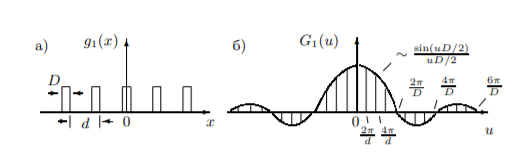
\includegraphics[width=0.9\textwidth]{teor1}
\end{center}
\ECaption{а) $g_1(x)$ — функция пропускания дифракционной решётки (последовательности прозрачных и непрозрачных полос);\\
б) $G_1(u)$ — спектр функции пропускания дифракционной решётки}
\end{figure}
а распределение амплитуд в
спектре (огибающая) — фурье-образом функции пропускания отдельного штриха:
\begin{equation}
g_2(x) = 
 \begin{cases}
   1 &\text{ при } -D/2\leq x \leq D/2\\
   0 &\text{ при } -D/2 > x \text{ и } x > D/2
 \end{cases}
\end{equation}
 Так
как функция
$g_2(x)$ непериодична, её фурье-образ представляется
непрерывным множеством точек
и определяется интегральным преобразованием Фурье:
\[g(x) = \frac{1}{2\pi}\int\limits_{-\infty}^{+\infty}G(u)e^{iux}du,\]
\[G(u) = \int\limits_{-\infty}^{+\infty}g(x)e^{-iux}dx.\]

 $G(u)$ — спектр или фурье-образ функции
$g(x)$.
Спектр функции
$g_2(x)$ хорошо известен, он соответствует
картине
дифракции Фраунгофера на щели
и описывается функцией вида $ \frac{\sin x}{x} $.

Получим спектр
$G_2(u)$ ещё раз с помощью преобразования Фурье:
\[G_2(u) = \int\limits_{-\infty}^{+\infty}g_2(x)e^{-iux}dx = \int\limits_{-\frac{D}{2}}^{+\frac{D}{2}}e^{-iux}dx = D sinc(\frac{uD}{2}).\]

Если ввести
понятия протяжённости функции пропускания транспаранта по
координате ($\Delta x$) и ширины её спектра ($ \Delta u $), то получаем соотношение неопределенности:

\[\Delta u \cdot \Delta x = const =2\pi.\]

\section*{Определение ширины щели}
\subsection*{Определение ширины щели с помощью линзы}

В этом этапе работы была посчитана ширина щели с помощью метода Аббе, изображенного на рис.2. 
\begin{figure}[h!]
\begin{center}
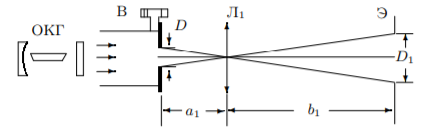
\includegraphics[width=0.7\textwidth]{ust1}
\end{center}
\ECaption{Схема для определения ширины щели с помощью линзы.}
\end{figure}

Использовалась линза с фокусным расстоянием $F_1 = 25$ мм. Известны $a_1=F_1$ и $b_1=132.3$ см. Таким образом из геометрической оптики получаем увеличение изображения сфокусированной линзы:
\[\Gamma = \frac{b_1}{a_1} = 52.92.\]

Эксперимент заключался в том, что с помощью макрометрического винта, можно менять ширину щели, а так же измерять эту самую ширину $d$. Однако это измерение не вполне точно из-за механики винта. Поэтому можно измерить ширину щели $D_{\text{л}}$ точнее с помощью размера изображения $D$:
\[\frac{D_{\text{л}}}{D} = \frac{1}{\Gamma}.\] 

Получаем таблицу с интересующими значениями.

\begin{table}[h!]
\begin{center}
\begin{tabular}{|c|c|c|}
\hline
\rowcolor[HTML]{9698ED} 
$d$, мкм & $D$, мм & $D_{\text{л}}$, мкм \\ \hline
90       & 5       & 94                  \\ \hline
\rowcolor[HTML]{9698ED} 
190      & 11      & 208                 \\ \hline
290      & 15      & 283                 \\ \hline
\rowcolor[HTML]{9698ED} 
390      & 22      & 416                 \\ \hline
490      & 26      & 491                 \\ \hline
\rowcolor[HTML]{9698ED} 
590      & 32      & 605                 \\ \hline
690      & 37      & 699                 \\ \hline
\rowcolor[HTML]{9698ED} 
790      & 45      & 850                 \\ \hline
890      & 51      & 964                 \\ \hline
\rowcolor[HTML]{9698ED} 
990      & 57      & 1077                \\ \hline
\end{tabular}
\ECaption{Таблица с зависимостью между показаниями винта, и значениями, измеренными методом линз. Цд винта -- 10 мкм.}
\end{center}
\end{table}
\newpage
\subsection*{Определение ширины щели по её спектру}

Метод определения ширины щели по спектру (рис.3) позволяет точнее измерить ширину очень узких щелей, когда изображение не превышает 10-15 мм. 

\begin{figure}[h!]
\begin{center}
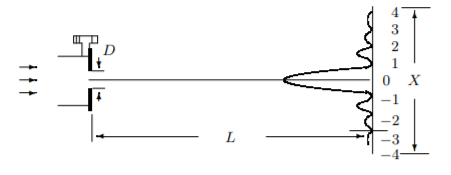
\includegraphics[width=0.7\textwidth]{ust2}
\ECaption{Схема для определения ширины щели по спектру. \\ Длина волны He-Ne лазера $\lambda = 632.8$ нм, $L = 135.8$ см.}
\end{center}
\end{figure}

Ширина щели $D_c$ была определена после серии измерений $X(m)$ -- расстояния между m-ми семмитричными максимумами, с помощью данных соотношений:
\[\Delta X = \frac{X}{2m} = \frac{\lambda}{D_c}L.\]

Так же для интереса этим же методом была измерена толщина волоса. Данные измерений $X(m)$ представлены на таблице 2. 

\begin{table}[h!]
\begin{center}
\begin{tabular}{|c|c|c|c|c|}
\hline
\rowcolor[HTML]{00D2CB} 
$d$, мкм & 110     & 170     & 250     & волос:                   \\ \hline
\rowcolor[HTML]{9698ED} 
$m$      & $X$, мм & $X$, мм & $X$, мм & $X$, мм                  \\ \hline
1        & 18      & 10      & 7       & 22                       \\ \hline
\rowcolor[HTML]{9698ED} 
2        & 33      & 20      & 14      & 43                       \\ \hline
3        & 48      & 30      & 20      & 66                       \\ \hline
\rowcolor[HTML]{9698ED} 
4        & 60      & 39      & 27      & 86                       \\ \hline
5        & 75      & 48      & 33      & 110                      \\ \hline
\rowcolor[HTML]{9698ED} 
6        & 90      & 57      & 40      & \cellcolor[HTML]{00D2CB} \\ \hline
\end{tabular}
\ECaption{Столбцы $X$ соответствуют ширине щели, измеренной винтом, находящейся выше, а так же волосу. Представленные ширины щелей примерно соответствуют области, в которой удалось засечь спектр.}
\end{center}
\end{table}

Построив графики для этих зависимостей (рис.4), получаем $D_c$.
\begin{figure}[h!]
\begin{center}
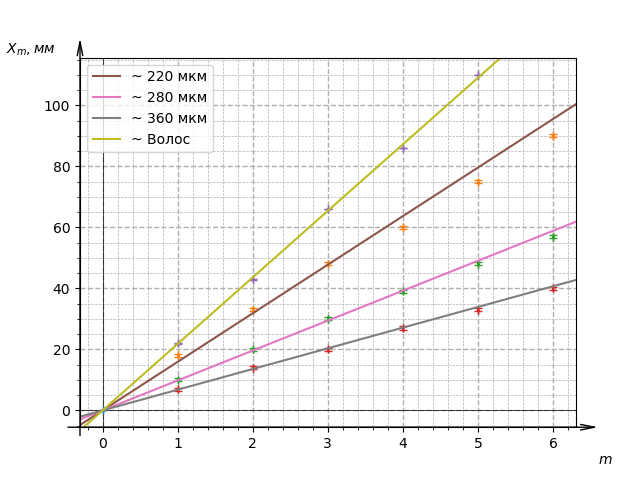
\includegraphics[width=0.7\textwidth]{gr1}
\ECaption{Графики $X(m)$. Из теории известно, что они должны проходить через начало координат, так что эта точка была добавлена в МНК.}
\end{center}
\end{figure}

Толщина волоса оказалась равной $78.3\pm0.6$ мкм. Это достаточно тонкий волос, так как средняя толщина волос человека колеблется в пределах 80-110 мкм, так что экспериментаторам стоит посоветовать шампунь для тонких волос.

По полученным значениям построены графики $D_{\text{л}}=f(d)$, $D_c = f(d)$,  чтобы показать достоверность измерений (рис.5).
\newpage
\begin{figure}[h!]
\begin{center}
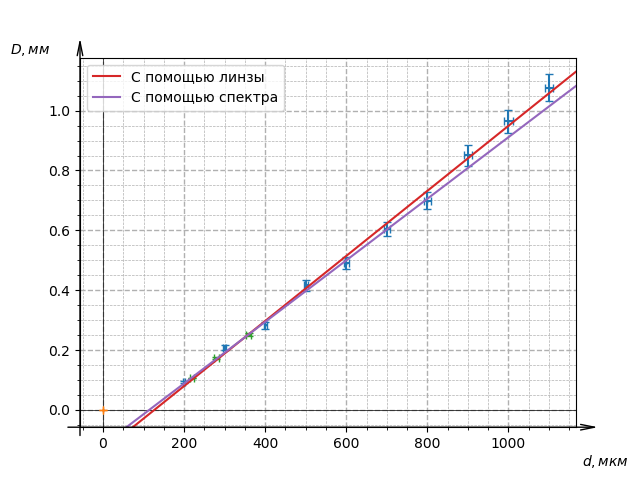
\includegraphics[width=0.7\textwidth]{gr2}
\ECaption{Этот график демонстрирует основные результаты данного пункта. Явным образом открывая щель, мы определяли, что ноль на винте сбит на 11 дел.. По графику же можно определить, что эта величина от 11 до 13 дел. С достаточно хорошей точностью угловой коэффициент обоих графиков близок к 1. ($1.09\pm 0.02$ (мнк занижает погрешность) для линзы и $1.03\pm 0.04$ для спектра)}
\end{center}
\end{figure}

\section*{Определение периода решеток}
\subsection*{Определение периода по спектру на удалённом экране}

Определить период решеток $d_c$ позволяет метод, аналогичный определению ширины щели по спектру. Однако вместо щели перед лазером ставится кассета с 5 разными сетками. Расстояние $L$ от кассеты до экрана равно 134.7 см. Снималась зависимость $X(m)$, из которой с помощью соотношений
\[\Delta X = \frac{X}{2m} = \frac{\lambda}{d_c}L,\]
можно определить период.

Строить графики в данном случае не имеет особого смысла, так как погрешность, определяемая МНК не будет сильно меньше погрешности, определенной по крайним точкам. Результаты представлены на таблице 3.
\newpage
\begin{table}[h!]
\begin{center}
\begin{tabular}{|c|c|c|c|c|c|}
\hline
\rowcolor[HTML]{00D2CB} 
Решетка:   & 1                        & 2                        & 3     & 4                        & 5                        \\ \hline
\rowcolor[HTML]{9698ED} 
m          & X, мм                    & X, мм                    & X, мм & X, мм                    & X, мм                    \\ \hline
1          & 72                       & 48                       & 24    & 12                       & 9                        \\ \hline
\rowcolor[HTML]{9698ED} 
2          & 144                      & 96                       & 48    & 24                       & 18                       \\ \hline
3          & 217                      & 144                      & 72    & 36                       & 26                       \\ \hline
\rowcolor[HTML]{9698ED} 
4          & \cellcolor[HTML]{DAE8FC} & 194                      & 97    & 48                       & 36                       \\ \hline
5          & \cellcolor[HTML]{DAE8FC} & 242                      & 121   & 60                       & 45                       \\ \hline
\rowcolor[HTML]{9698ED} 
6          & \cellcolor[HTML]{DAE8FC} & \cellcolor[HTML]{DAE8FC} & 145   & 72                       & 54                       \\ \hline
7          & \cellcolor[HTML]{DAE8FC} & \cellcolor[HTML]{DAE8FC} & 169   & \cellcolor[HTML]{DAE8FC} & \cellcolor[HTML]{DAE8FC} \\ \hline
\rowcolor[HTML]{00D2CB} 
$d_c$, мкм & 23                       & 35                       & 70    & 142                      & 188                      \\ \hline
\end{tabular}
\ECaption{Значения периодов решетки, померянные без увеличения.}
\end{center}
\end{table}

\subsection*{Определение периода решёток по увеличенному изображению спектра}

Для определения периода крупных решеток предпочтительнее увеличивать изображение спектра с помощью схемы, представленной на рис.6.
\begin{figure}[h!]
\begin{center}
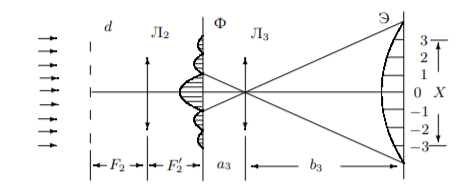
\includegraphics[width=0.7\textwidth]{ust3}
\ECaption{Схема определения периода решётки по увеличенному
изображению спектра. \\
$F_2 = 110$ мм, $a_3 = 25$ мм, $b_3 = L - 2F_2 - a_3$. \\ Таким образом получаем значение для увеличения: $\Gamma_3 = 43.41$. }
\end{center}
\end{figure}

Рассчет в данном случае происходит по этой формуле, где $\Delta x$ -- расстояние между максимумами в фокальной плоскости Ф:
\[\Delta x = \frac{\Delta X}{\Gamma_3} = \frac{\lambda}{d_{\text{л}}}F_2.\]

Результаты на таблице 4. 
\newpage

\begin{table}[h!]
\begin{center}
\begin{tabular}{|c|c|c|c|c|c|}
\hline
\rowcolor[HTML]{00D2CB} 
Решетка:                              & 1                        & 2                        & 3                        & 4                        & 5     \\ \hline
\rowcolor[HTML]{9698ED} 
m                                     & X, мм                    & X, мм                    & X, мм                    & X, мм                    & X, мм \\ \hline
1                                     & \cellcolor[HTML]{DAE8FC} & 195                      & 98                       & 49                       & 37    \\ \hline
\rowcolor[HTML]{9698ED} 
2                                     & \cellcolor[HTML]{DAE8FC} & \cellcolor[HTML]{DAE8FC} & 197                      & 97                       & 73    \\ \hline
3                                     & \cellcolor[HTML]{DAE8FC} & \cellcolor[HTML]{DAE8FC} & \cellcolor[HTML]{DAE8FC} & 148                      & 109   \\ \hline
\rowcolor[HTML]{9698ED} 
4                                     & \cellcolor[HTML]{DAE8FC} & \cellcolor[HTML]{DAE8FC} & \cellcolor[HTML]{DAE8FC} & 197                      & 146   \\ \hline
5                                     & \cellcolor[HTML]{DAE8FC} & \cellcolor[HTML]{DAE8FC} & \cellcolor[HTML]{DAE8FC} & \cellcolor[HTML]{DAE8FC} & 188   \\ \hline
\rowcolor[HTML]{00D2CB} 
d\_\{\textbackslash{}text\{л\}\}, мкм & --                       & 31                       & 61                       & 123                      & 163   \\ \hline
\end{tabular}
\ECaption{К сожалению, на первой кассете поймать даже первый максимум не удалось --- картина слишком широкая.}
\end{center}
\end{table}

\section*{Мультиплицирование}

Для наблюдения мультиплицирования (рис.7) перед лазером была поставлена щель, и линза Л$_2$. В фокальной плоскости
Ф линзылена
кассета с сетками,
которые будут «рассекать» фурье-образ щели
— осуществлять пространственную фильтрацию.

\begin{figure}[h!]
\begin{center}
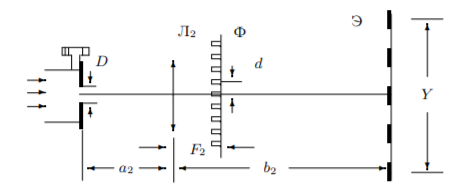
\includegraphics[width=0.6\textwidth]{ust4}
\ECaption{Схема для наблюдения мультиплицирования. $D = 30$ дел. }
\end{center}
\end{figure}

К сожалению, в лаборатории не были измерены значения $a_2$ и $b_2$, однако нам известно, что $a_2+b_2=L$, а также известно, что:
\[\frac{1}{a_2}+\frac{1}{b_2}=\frac{1}{F_2},\]
потому что изначально без решётки Ф линза фокусировала изображение щели на экран Э. Решая систему этих несложных уравнений и вспоминая,что линза была ближе к щели, чем к экрану, получаем: $a_2=120.8 \pm 1.2$ мм, $b_2=1230 \pm 10$ мм. Таким образом находим увеличение $\Gamma_2 = 10.18$.

Была снята зависимость
$Y$ (расстояние между
удалёнными изображениями
щели)
и
$K$ (число промежутков между изображениями) от номера сетки для фиксированной ширины входной щели.

Для периода "фиктивной" решетки имеем:
\[\Delta y = \frac{\Delta Y}{\Gamma_2} = \frac{Y}{K\Gamma_2}.\]

Зависимость $Y(K)$ показана на таблице 5.
\begin{table}[h!]
\begin{center}
\begin{tabular}{|c|c|c|c|c|c|}
\hline
\rowcolor[HTML]{00D2CB} 
Решетка: & 1                        & 2                        & 3                        & 4                        & 5                        \\ \hline
\rowcolor[HTML]{9698ED} 
K        & Y, мм                    & Y, мм                    & Y, мм                    & Y, мм                    & Y, мм                    \\ \hline
1        & 30                       & \cellcolor[HTML]{DAE8FC} & 10                       & 5                        & \cellcolor[HTML]{DAE8FC} \\ \hline
\rowcolor[HTML]{9698ED} 
2        & 60                       & 40                       & 20                       & 10                       & 7                        \\ \hline
3        & 90                       & 59                       & \cellcolor[HTML]{DAE8FC} & \cellcolor[HTML]{DAE8FC} & 15                       \\ \hline
\rowcolor[HTML]{9698ED} 
4        & 119                      & 79                       & 40                       & 20                       & 21                       \\ \hline
6        & 180                      & 118                      & 60                       & 30                       & 30                       \\ \hline
\rowcolor[HTML]{9698ED} 
8        & \cellcolor[HTML]{DAE8FC} & 158                      & 80                       & 40                       & 39                       \\ \hline
10       & \cellcolor[HTML]{DAE8FC} & \cellcolor[HTML]{DAE8FC} & \cellcolor[HTML]{DAE8FC} & 50                       & \cellcolor[HTML]{DAE8FC} \\ \hline
\end{tabular}
\ECaption{Зависимость $Y(K)$.}
\end{center}
\end{table}

Теперь осталось построить график
$ \Delta y = f(\frac{1}{d_c}) $ (рис. 8), где
$ d_c $ — периоды решёток, определённые по спектру. Зависимость должна быть линейной, поскольку
\[\frac{\lambda}{\Delta y} F_2 = d_c.\]

\begin{figure}[h!]
\begin{center}
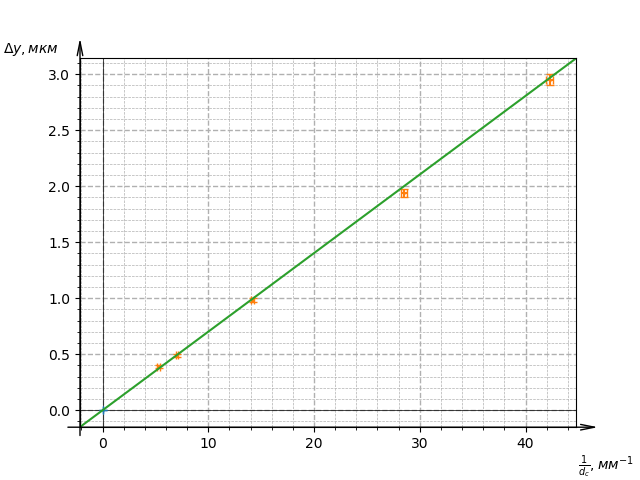
\includegraphics[width=1\textwidth]{gr3}
\ECaption{ График $ \Delta y = f(\frac{1}{d_c}) $. Как видно, он прямой. }
\end{center}
\end{figure}


\section*{Вывод}

Определение щели с помощью линзы и с помощью спектра даёт почти одни и те же результаты. Причина различия заключается в неровности самой щели. Спектр в окрестности нуля выдаёт эффективную величину, а линза и прямое измерение дают ширину щели в её самом узком месте. Проверка показала, что измерение толщины с помощью винта - достаточно точное. Так же, с помощью спектрального метода можно достоверно находить толщину крайне тонких объектов, вроде человеческого волоса.

 С помощью этого метода были определены периоды сеток с большей точностью, а методом мультиплицированиями мы показали, что измеренные значения периода достоверны.







\end{document}